\documentclass{beamer}
\usetheme{Madrid}
\usecolortheme{beaver}
\usepackage[utf8]{inputenc}
\usepackage[MeX]{polski}
%Information to be included in the title page:
\title{Mars - planeta}
\author{Marceli Sobiecki}
\institute[WMiI UWM]{Wydział Matematyki i Informatyki.\\
Uniwersytet Warmińsko-Mazurski w Olsztynie}
\date{\today}

\begin{document}
\maketitle


\begin{frame}
\frametitle{Podstawowe Informacje}

Mars jest \alert{czwartą planetą Układu Słonecznego}, a zarazem ostatnią planetą ziemską. Czasami jest także nazywany Czerwoną Planetą. Orbita Marsa jest bardziej eliptyczna niż orbita ziemska. Czerwona Planeta jest oddalona od Słońca o 228 milionów kilometrów. Swój kolor Mars zawdzięcza dużej zawartości w skorupie tlenków żelaza. Mars, obok Ziemi, ma najbardziej zróżnicowaną powierzchnię wśród wszystkich planet Układu Słonecznego.
\begin{block}{Ciekawostka}
Temperatura na marsie waha się od -130 stopni Celsjusza w okresie zimowym do +55 stopni w lecie.
\end{block}
\end{frame}

\begin{frame}
\frametitle{Parametry Marsa}
\begin{table}[h]
\centering
\begin{tabular}{|l|l|}
\hline
Ciało centralne & Słońce        \\ \hline
Półoś wielka    & $2,2792\times 10^{11}$ m \\ \hline
Obwód orbity    & $1,429$ Tm      \\ \hline
\end{tabular}
\caption{Dane o marsie}
\end{table}
\end{frame}

\begin{frame}
\frametitle{Zdjecie Marsa}
\begin{figure}[h]
\centering
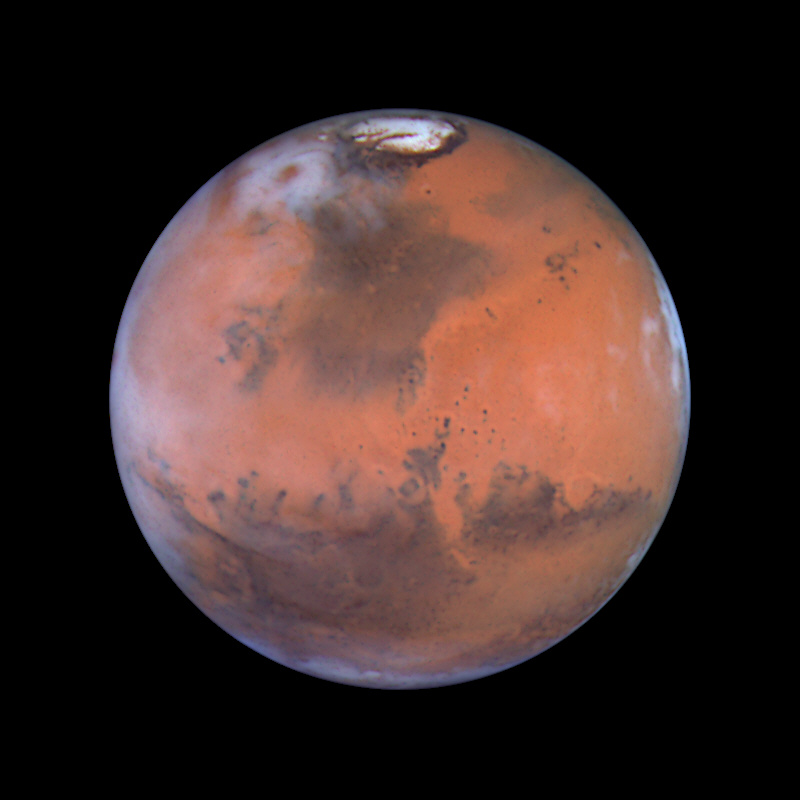
\includegraphics[width=0.4\textwidth]{mars.jpg}
\caption{widok Marsa.}
\end{figure}
\end{frame}

\begin{frame}
\frametitle{Twarz na marsie}
"Marsjańska Twarz" - tak przezwano jeden z tworów geologicznych na powierzchni Marsa. Trudno się temu dziwić, jeśli spojrzymy na fotografię wykonaną przez sondę orbitalną Viking 1 w dniu 25 lipca 1976 r. Czyżby to ślady jakiejś dawnej cywilizacji? Nic z tych rzeczy, jest to po prostu akurat taki układ cieni i ludzka wyobraźnia próbująca dopatrzeć się znajomych kształtów.

 
\begin{block}{Ciekawostka}
Struktura ma 3 km długości i 240 m wysokości. Zdjęcie tego samego tworu wykonane przez sondy Mars Global Surveyor w 2001 roku oraz w 2007 roku rozwiewają wątpliwości. 
\end{block}
\end{frame}

\begin{frame}
\frametitle{Twarz na marsie}
\begin{figure}[h]
\centering
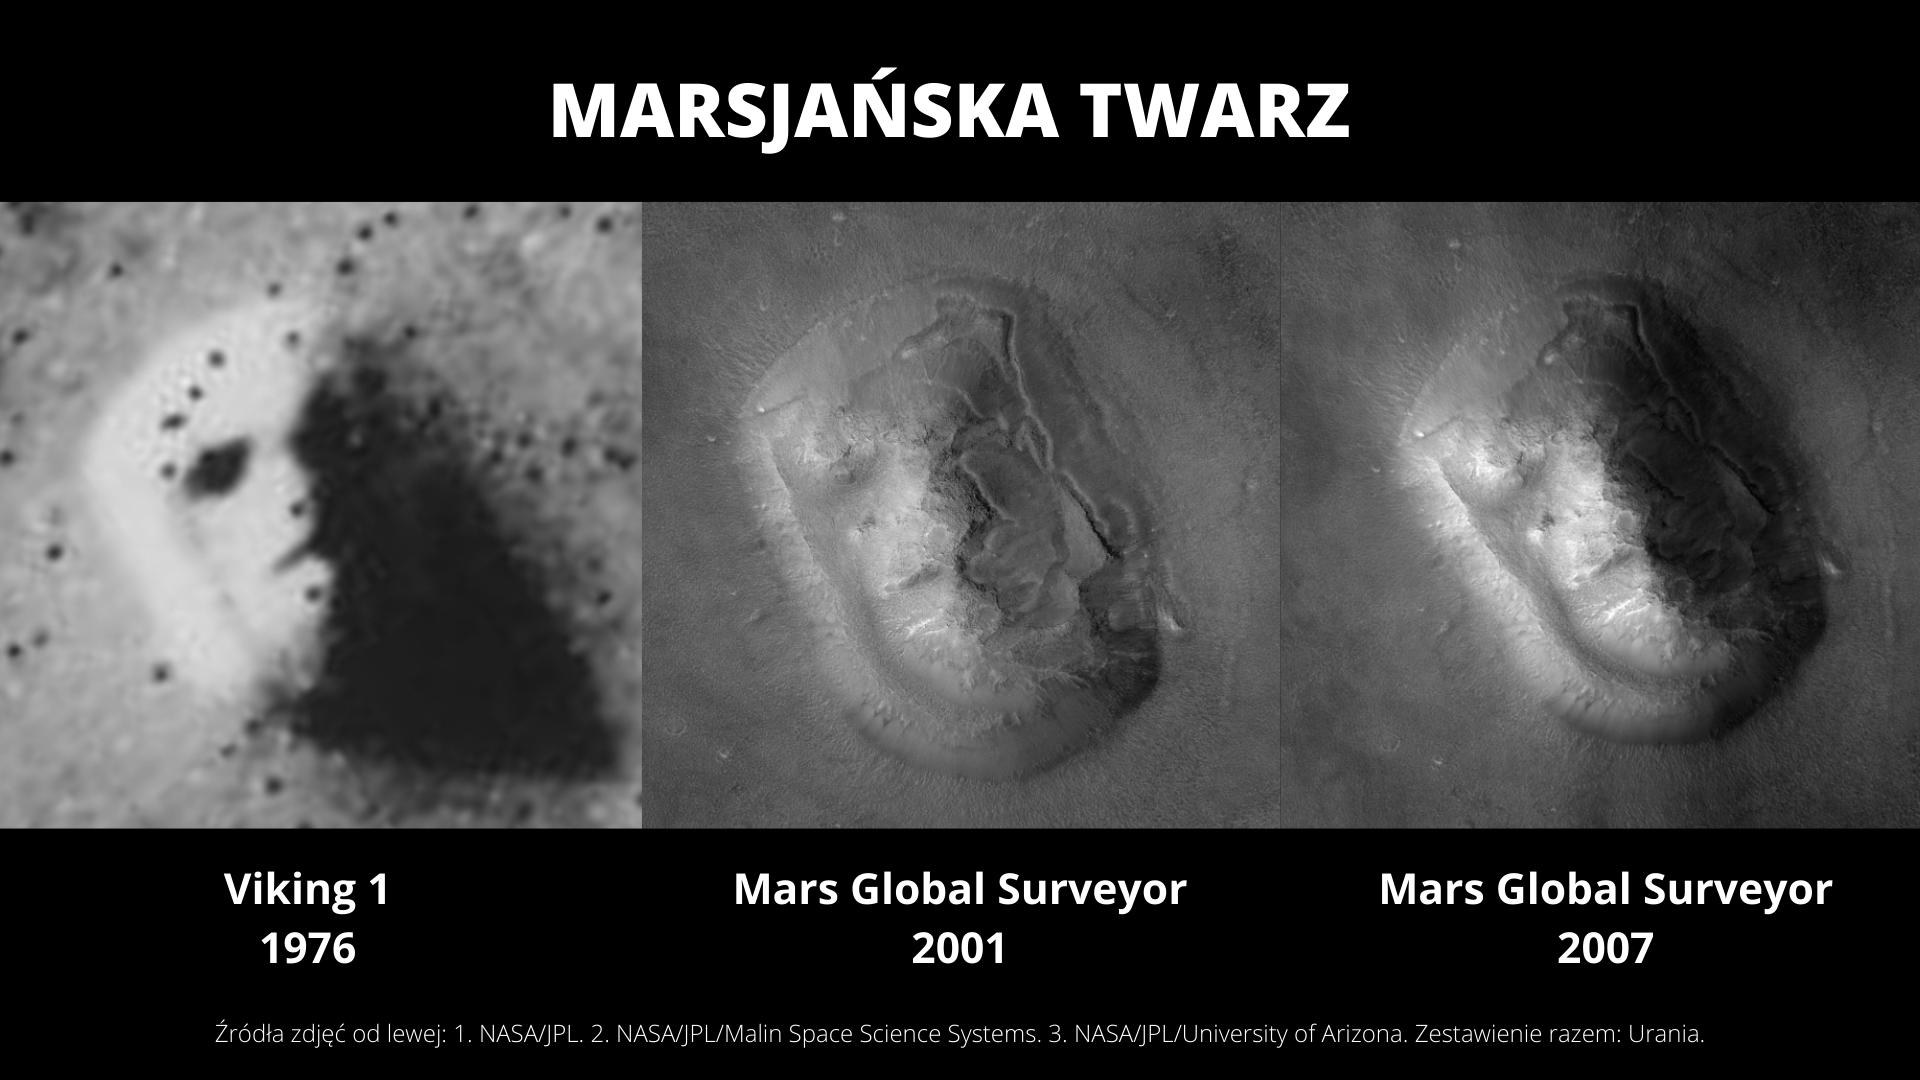
\includegraphics[width=1\textwidth]{twarz.png}
\end{figure}
\end{frame}

\begin{frame}
\frametitle{Na Marsie ważylibyśmy trzy razy mniej}
Stojąc na powierzchni Marsa nasz ciężar będzie mniejszy - ważylibyśmy zdecydowanie mniej niż na Ziemi, aż o 62 \% mniej! Czyli około trzykrotnie mniej. Wynika to z tego, że Mars ma około 10 razy mniejszą masę niż Ziemia, a więc wytwarza mniejsze przyciąganie grawitacyjne. Liczy się tu także promień planety, dlatego waga nie byłaby w prosty sposób dziesięć razy mniejsza, gdyż rozmiary Marsa to mniej więcej połowa rozmiarów Ziemi.

\begin{block}{Ciekawostka}
Czyli osoba ważąca na Ziemi przykładowo 70 kg, na Marsie ważyłaby 26 kg. Jeśli ważymy 50 kg, to na Marsie będzie to niecałe 19 kg, a w przypadku 100 kg wychodzi 38 kg.
\end{block}
\end{frame}

\begin{frame}
\frametitle{Waga na Marsie}
\begin{figure}[h]
\centering
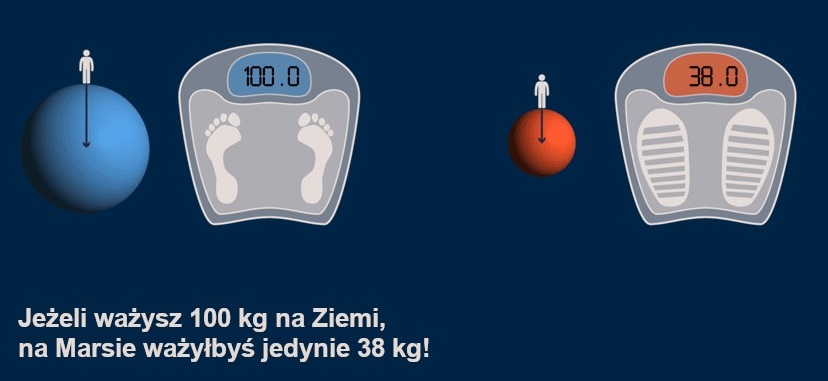
\includegraphics[width=1\textwidth]{waga.jpg}
\end{figure}
\end{frame}





\end{document}
